\documentclass[12pt]{report}
\usepackage[utf8]{inputenc}
\usepackage[english, russian]{babel}
\usepackage{listings}
\usepackage{graphicx}
\usepackage{float}
\graphicspath{{imgs/}}
\usepackage{amsmath,amsfonts,amssymb,amsthm,mathtools} 
\usepackage{pgfplots}
\usepackage{filecontents}
\usepackage{indentfirst}
\usepackage{eucal}
\usepackage{enumitem}
\frenchspacing

\usepackage{indentfirst} % Красная строка

\usetikzlibrary{datavisualization}
\usetikzlibrary{datavisualization.formats.functions}

\usepackage{amsmath}
\usepackage{fixltx2e}
\usepackage{caption}


\definecolor{bluekeywords}{rgb}{0,0,1}
\definecolor{greencomments}{rgb}{0,0.5,0}
\definecolor{redstrings}{rgb}{0.64,0.08,0.08}
\definecolor{xmlcomments}{rgb}{0.5,0.5,0.5}
\definecolor{types}{rgb}{0.17,0.57,0.68}

\usepackage{listings}
\lstset{language=[Sharp]C,
	captionpos=t,
	numbers=left, %Nummerierung
	numberstyle=\small, % kleine Zeilennummern
	frame=single, % Oberhalb und unterhalb des Listings ist eine Linie
	stepnumber=1,                   
	numbersep=5pt,                
	showspaces=false,
	tabsize=2,
	showtabs=false,
	breaklines=true,
	showstringspaces=false,
	breakatwhitespace=true,
	escapeinside={(*@}{@*)},
	commentstyle=\color{greencomments},
	morekeywords={partial, var, value, get, set},
	keywordstyle=\color{bluekeywords},
	stringstyle=\color{redstrings},
	basicstyle=\ttfamily\small,
}

\usepackage[left=2cm,right=2cm, top=2cm,bottom=2cm,bindingoffset=0cm]{geometry}
% Для измененных титулов глав:
\usepackage{titlesec, blindtext, color} % подключаем нужные пакеты
\definecolor{gray75}{gray}{0.75} % определяем цвет
\newcommand{\hsp}{\hspace{20pt}} % длина линии в 20pt
% titleformat определяет стиль
\titleformat{\chapter}[hang]{\Huge\bfseries}{\thechapter\hsp\textcolor{gray75}{|}\hsp}{0pt}{\Huge\bfseries}

\usepackage{array}
\newcommand{\head}[2]{\multicolumn{1}{>{\centering\arraybackslash}p{#1}}{#2}}

% plot
\usepackage{pgfplots}
\usepackage{filecontents}
\usetikzlibrary{datavisualization}
\usetikzlibrary{datavisualization.formats.functions}
 
\begin{document}
  %\def\chaptername{} % убирает "Глава"
\thispagestyle{empty}
\begin{titlepage}
	\noindent \begin{minipage}{0.15\textwidth}
	
\includegraphics[width=\linewidth]{b_logo}
	\end{minipage}
	\noindent\begin{minipage}{0.9\textwidth}\centering
		\textbf{Министерство науки и высшего образования Российской Федерации}\\
		\textbf{Федеральное государственное бюджетное образовательное учреждение высшего образования}\\
		\textbf{~~~«Московский государственный технический университет имени Н.Э.~Баумана}\\
		\textbf{(национальный исследовательский университет)»}\\
		\textbf{(МГТУ им. Н.Э.~Баумана)}
	\end{minipage}
	
	\noindent\rule{18cm}{3pt}
	\newline\newline
	\noindent ФАКУЛЬТЕТ $\underline{\text{«Информатика и системы управления»}}$ \newline\newline
	\noindent КАФЕДРА $\underline{\text{«Программное обеспечение ЭВМ и информационные технологии»}}$\newline\newline\newline\newline\newline\newline\newline\newline\newline\newline\newline
	
	
	\begin{center}
		\noindent\begin{minipage}{1.3\textwidth}\centering
			\Large\textbf{  Отчет по лабораторной работе №4}\newline
			\textbf{по дисциплине "Анализ алгоритмов"}\newline\newline
		\end{minipage}
	\end{center}
	
	\noindent\textbf{Тема} $\underline{\text{Исследование многопоточности}}$\newline\newline
	\noindent\textbf{Студент} $\underline{\text{Малышев И. А.}}$\newline\newline
	\noindent\textbf{Группа} $\underline{\text{ИУ7-51Б}}$\newline\newline
	\noindent\textbf{Оценка (баллы)} $\underline{\text{~~~~~~~~~~~~~~~~~~~~~~~~~~~}}$\newline\newline
	\noindent\textbf{Преподаватель: } $\underline{\text{Волкова Л. Л.}}$\newline\newline\newline
	
	\begin{center}
		\vfill
		Москва~---~\the\year
		~г.
	\end{center}
\end{titlepage}


\renewcommand{\contentsname}{Содержание}
\tableofcontents
  
\newpage
\chapter*{Введение}
\addcontentsline{toc}{chapter}{Введение}

Поток, или поток выполнения, -- базовая упорядоченная последовательность инструкций, которые могут быть переданы или обработаны одним ядром процессора. Вычисления разбиваются на части, за каждую из которых отвечает отдельный поток. Если в системе больше одного процессора, то использование многопоточности фактически позволяет выполнять несколько действий одновременно.

Многие алгоритмы (операции над матрицами, алгоритмы сортировки и т. д.) допускают многопоточную реализацию. Поэтому \textbf{целью} данной работы является сравнить производительность обычной и многопоточной реализаций алгоритма вычисления среднего степенного для строк матрицы.
Для достижения поставленной цели необходимо решить следующие задачи:
\begin{itemize}
	\item изучить стандартный алгоритм вычисления среднего степенного для строк матрицы и найти способ его распараллеливания;
	\item разработать и привести схемы алгоритмов;
	\item выбрать средства реализации;
	\item реализовать однопоточный и многопоточный алгоритм вычисления среднего степенного для строк матрицы;
	\item протестировать реализованные алгоритмы;
	\item провести сравнительный анализ алгоритмов на основе экспериментальных данных о времени выполнения в зависимости от количества потоков.
\end{itemize}


\chapter{Аналитическая часть}

В этом разделе приведён обзор и анализ алгоритмов вычисления среднего степенного для строк матрицы.

\section{Стандартный алгоритм}

Пусть дана прямоугольная матрица
\begin{equation}
	A_{nm} = \begin{pmatrix}
		a_{11} & a_{12} & \ldots & a_{1m}\\
		a_{21} & a_{22} & \ldots & a_{2m}\\
		\vdots & \vdots & \ddots & \vdots\\
		a_{l1} & a_{l2} & \ldots & a_{nm}
	\end{pmatrix},
\end{equation}
тогда вектор $B$
\begin{equation}
	B_{n} = \begin{pmatrix}
		b_{1} & b_{2} & \ldots & b_{n}\\
	\end{pmatrix},
\end{equation}
где
\begin{equation}
	\label{eq:M}
	b_{i} = \sqrt[d]{\frac{\sum_{j=1}^{m} a_{ij} ^ d}{m}} \quad, (j=\overline{1,m})
\end{equation}
будет называться средним степенным строки матрицы $A$ [1].

\section{Параллельный алгоритм}

Можно заметить, что каждый элемент вектора $B$ вычисляется независимо от других и матрица $A$ не изменяется. Тогда для параллельного вычисления среднего степенного строк достаточно просто равным образом распределить строки матрицы $A$ между потоками [2].

\section{Вывод}

В данном разделе было выявлено, что обычный алгоритм получения среднего степенного от ряда чисел в строке матрицы независимо вычисляет элементы вектора-результата, что дает большое количество возможностей для реализации параллельного варианта алгоритма.

\newpage

\chapter{Конструкторская часть}

В этом разделе приводятся схемы алгоритмов вычисления среднего степенного для строк матрицы, приведённых в аналитической части. 

\section{Схемы алгоритмов}

На рисунках \ref{std} и \ref{prl} показаны схемы алгоритмов сортировки пузырьком, выбором и быстрой сортировки соответственно.

\begin{figure}[H]
	\centering
	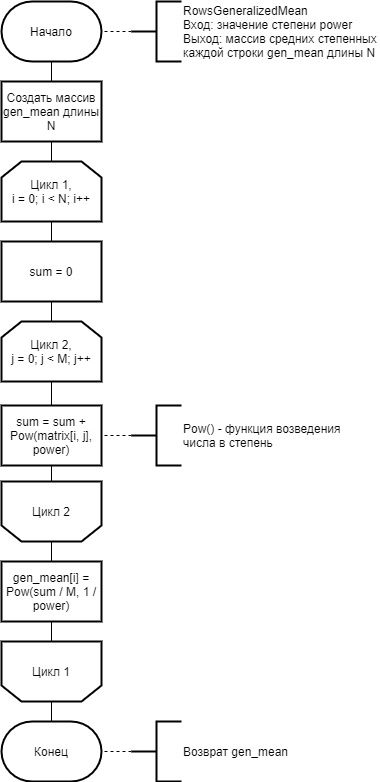
\includegraphics[scale = 0.5]{standart_scheme.png}
	\caption{Схема стандартного алгоритма}
	\label{std}
\end{figure}

\begin{figure}[H]
	\centering
	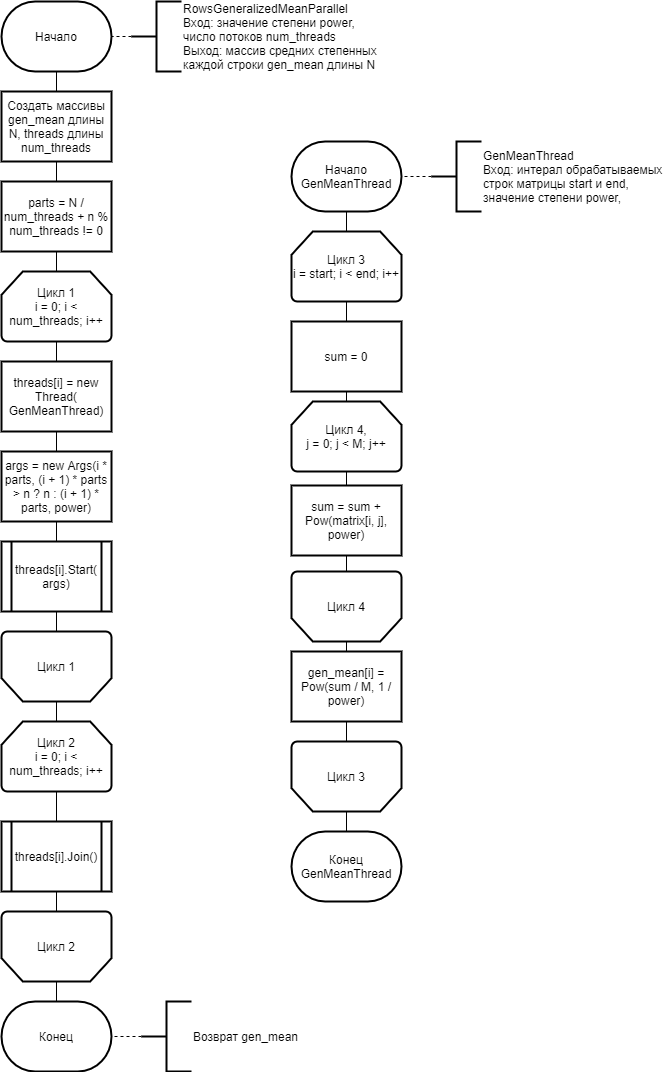
\includegraphics[scale = 0.52]{parallel_scheme.png}
	\caption{Схема параллельной версии алгоритма}
	\label{prl}
\end{figure}

\section{Вывод}
На основе теоретических данных, полученных из аналитического раздела, были построены схемы алгоритмов вычисления среднего степенного для строк матрицы.

\newpage

\chapter{Технологическая часть}
В данном разделе приводится реализация алгоритмов, схемы которых были разработаны в конструкторской части. Кроме того, обосновывается выбор технологического стека и проводится тестирование реализованных алгоритмов.

\section{Средства реализации}

В качестве языка программирования был выбран C\#, а среды разработки -- Visual Studio, т. к. я знаком с данным языком и имею представление о тестировании программ в данном языке. Время работы алгоритмов было замерено с помощью библиотеки System.Diagnostics, класса Stopwatch, который имеет методы для расчёта процессорного времени [3].


\section{Реализация алгоритмов}

В листингах 3.1 и 3.2 приведена реализация стандартного и параллельного алгоритмов вычисления среднего степенного для строк матрицы.

\captionsetup{singlelinecheck = false, justification=raggedright}
\begin{lstlisting}[label=base_code,caption=Стандартный метод вычисления среднего степенного для строк матрицы]
public double[] RowsGenMean(double power)
{
	double[] gen_means = new double[n];
	
	for (int i = 0; i < n; i++)
	{
		double sum = 0;
		for (int j = 0; j < m; j++)
			sum += Math.Pow(matrix[i, j], power);
		
		gen_means[i] = Math.Pow(sum / m, 1.0 / power);
	}
	
	return gen_means;
}
\end{lstlisting}
\newpage
\begin{lstlisting}[label=vin_code,caption=Параллельный метод вычисления среднего степенного для строк матрицы]
public double[] RowsGenMeanParallel(double power, int num_threads = 1)
{
	Thread[] threads = new Thread[num_threads];
	double[] gen_means = new double[n];
	
	int parts = n / num_threads + (n % num_threads != 0 ? 1 : 0);
	
	for (int i = 0; i < num_threads; i++)
	{
		threads[i] = new Thread(GenMeanThread);
		
		Args args = new Args(i * parts, (i + 1) * parts > n ? n : (i + 1) * parts, power);
		
		threads[i].Start(args);
	}
	
	foreach (Thread t in threads)
		t.Join();
	
	return gen_means;
	
	void GenMeanThread(object obj)
	{
		Args args = (Args)obj;
		var (start, end) = (args.row_indx_start, args.row_indx_end);
		double pow = args.power;
		
		for (int i = start; i < end; i++)
		{
			double sum = 0;
			for (int j = 0; j < m; j++)
				sum += Math.Pow(matrix[i, j], pow);
			
			gen_means[i] = Math.Pow(sum / m, 1.0 / pow);
		}
	}
}
\end{lstlisting}
\captionsetup{singlelinecheck = false, justification=centering}

\newpage

\section{Тестирование}

В таблице~\ref{tabular:test} приведены тесты для функций, реализующих стандартный и параллельный алгоритм вычисления среднего степенного для строк матрицы. Число потоков для многопоточной версии равно числу строк в матрице.

\begin{table}[H]
	\begin{center}
		\caption{\label{tabular:test} Тестирование функций}
		\begin{tabular}{c c c c c}
			\hline
			\head{2.0cm}{Матрица} & \head{1.0cm}{Степень} & \head{4cm}{Ожидаемый результат} & \head{4cm}{Фактический результат (стандартный)} & \head{4cm}{Фактический результат (многопоточный)}\\
			\hline
			\vspace{4mm}
			$\begin{pmatrix}
				1 & 2 & 3\\
				3 & 4 & 5
			\end{pmatrix}$ &
			2 &
			$\begin{pmatrix}
				2.1602 & 4.0825 
			\end{pmatrix}$ &
			$\begin{pmatrix}
				2.1602 & 4.0825 
			\end{pmatrix}$ &
			$\begin{pmatrix}
				2.1602 & 4.0825 
			\end{pmatrix}$ \\
			\vspace{4mm}
			$\begin{pmatrix}
				1 & 2\\
				3 & 4\\
				5 & 6
			\end{pmatrix}$ &
			0.5 &
			$\begin{pmatrix}
				1.4571 & 3.4821 & 5.4886
			\end{pmatrix}$ &
			$\begin{pmatrix}
				1.4571 & 3.4821 & 5.4886
			\end{pmatrix}$ &
			$\begin{pmatrix}
				1.4571 & 3.4821 & 5.4886
			\end{pmatrix}$ \\
			\vspace{4mm}
			$\begin{pmatrix}
				2
			\end{pmatrix}$ &
			1 &
			$\begin{pmatrix}
				2
			\end{pmatrix}$ &
			$\begin{pmatrix}
				2
			\end{pmatrix}$ &
			$\begin{pmatrix}
				2
			\end{pmatrix}$ \\
			\vspace{4mm}
			$\begin{pmatrix}
				1 & 2 & 3\\
				4 & 5 & 6\\
				7 & 8 & 9
			\end{pmatrix}$ &
			0 &
			$\begin{pmatrix}
				1 & 1 & 1
			\end{pmatrix}$ &
			$\begin{pmatrix}
				1 & 1 & 1
			\end{pmatrix}$ &
			$\begin{pmatrix}
				1 & 1 & 1
			\end{pmatrix}$ \\
		\end{tabular}
	\end{center}
\end{table}
Все тесты пройдены успешно.
\section{Вывод}

В данном разделе были реализованы стандартный и параллельный алгоритм вычисления среднего степенного для строк матрицы. Кроме того, реализации были успешно протестированы.

\newpage

\chapter{Исследовательская часть}

В данном разделе проводится сравненительный анализ реализованных алгоритмов по процессорному времени.

\section{Технические характеристики}

Ниже приведены технические характеристики устройства, на котором было проведено тестирование ПО:

\begin{itemize}
	\item операционная система: Windows 10 Home 64-bit [4];
	\item оперативная память: 16 ГБ;
	\item процессор: 4.0 GHz 4‑ядерный процессор Intel Core i7-4790K [5].

\end{itemize}

\section{Время выполнения реализаций алгоритмов}

Для сравнительного анализа времени выполнения реализаций алгоритмов были проведены эксперименты. Для замеров были сформированы следующие данные:
\begin{itemize}
	\item матрица со случайными числами размером 1024 на 1024;
	\item значение степени равно 2.
\end{itemize}

В таблице \ref{time1} представлены результаты замеров. Время измерялось 100 раз для каждого числа потоков, после усреднялось. 

\begin{table} [H]
	\label{time1}
	\caption{Таблица времени выполнения (в тиках) алгоритмов при разном числе потоков}
	\begin{center}
		\begin{tabular}{|c c|} 
			\hline
			Число потоков & Время выполнения \\  
			\hline
			не распараллелено & 455 547 \\
			\hline
			1 & 549 188 \\
			\hline
			2 & 369 247 \\
			\hline
			4 & 221 466 \\
			\hline
			8 & 218 486 \\
			\hline
			16 & 243 658 \\
			\hline
			32 & 248 079 \\
			\hline
		\end{tabular}
	\end{center}
\end{table}

\section{Вывод}

На основе замеров процессорного времени было получено, что на конкретных данных параллельный алгоритм имеет наименьшее время работы при 8 потоках, что соответствует числу логических ядер компьютера, на котором проводилось тестирование. При числе потоков больше 8 увеличивается время работы алгоритма на тестируемом компьютере. Таким образом, рекомендуется использовать число потоков, равное числу логических ядер.

Также выявлено, что параллельная реализация при 8 потоках быстрее стандарной примерно в 2.1 раза. Хотя не распараллеленная реализация имеет меньшее время работы по сравнению с однопоточной, поскольку в однопоточной уходит время на создание потока.


\chapter*{Заключение}
\addcontentsline{toc}{chapter}{Заключение}

В рамках данной лабораторной работы:

\begin{itemize}
	\item был найден способ распараллеливания алгоритма вычисления среднего степенного для строк матрицы;
	\item были разработаны и приведены схемы алгоритмов;
	\item были реализованы однопоточный и многопоточный алгоритм вычисления среднего степенного для строк матрицы, а также протестированы;
	\item был проведён сравнительный анализ алгоритмов на основе экспериментальных данных: по времени выполнения в зависимости от количества потоков.
\end{itemize}

В результате исследования было выяснено, что параллельные реализации алгоритма вычисления среднего степенного для строк матрицы работают быстрее стандартной реализации. Наиболее эффективны данные алгоритмы при количестве потоков, совпадающем с количеством логических ядер компьютера. Так, на матрице размером 1024 на 1024 удалось улучшить время выполнения алгоритма в 2.1 раз (в сравнении со стандартной реализацией).

Поставленная цель была достигнута.

\chapter*{Список литературы}
\addcontentsline{toc}{chapter}{Список литературы}
\begin{enumerate}
	\item Математическое просвещение (II). Выпуск 6. Математика, ее преподавание, приложения и история. Сборник. - М., ГИТТЛ, 1961. 376 с.
	\item Kunle Olukotun. Chip Multiprocessor Architecture - Techniques to Improve Throughput and Latency. — Morgan and Claypool Publishers, 2007. — 154 p.
	\item Свойство Process.UserProcessorTime [Электронный ресурс]. Режим доступа: https://docs.microsoft.com/ru-ru/dotnet/api/system.diagnostics.stopwatch?view=net-5.0. Дата обращения: 26.10.2021
	\item Windows 10 [Электронный ресурс]. Режим доступа: https://www.microsoft.com/ru-ru/windows/get-windows-10. Дата обращения: 26.10.2021
	\item Процессор Intel Core I7-4790K [Электронный ресурс]. Режим доступа: https://ark.intel.com/content/www/ru/ru/ark/products/80807/intel-core-i7-4790k-processor-8m-cache-up-to-4-40-ghz.html. Дата обращения: 26.10.2021
\end{enumerate}


\end{document}